 \scalebox  {0.7} {
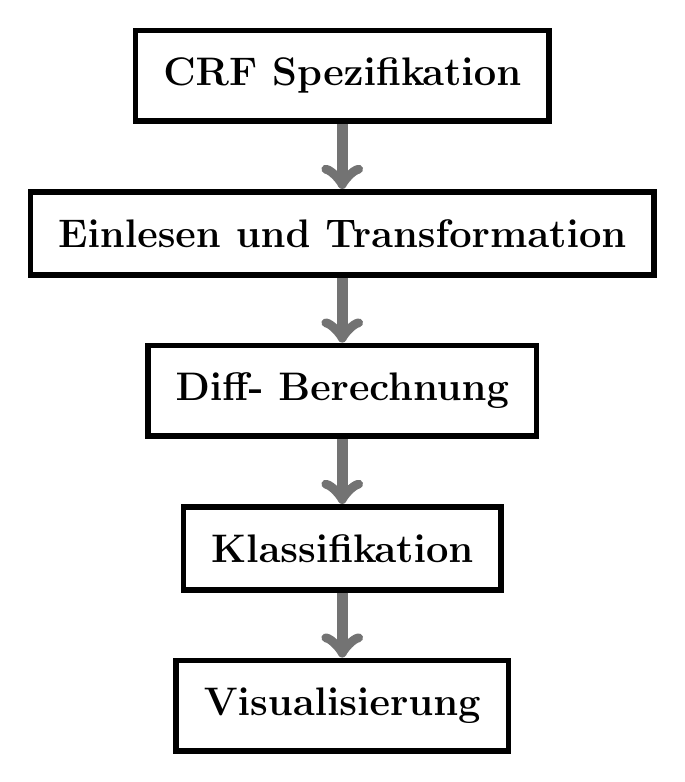
\begin{tikzpicture}

\tikzstyle{mynodestyle} = [draw,font={\Large\bfseries},line width=2,outer sep=1,inner sep=10,minimum size=10]
\tikzstyle{green_arrow_edge} = [->, draw=black!55, line width=4pt]
  

\node [mynodestyle] (v1) at (-18,12) {CRF Spezifikation};
\node [mynodestyle] (v2) at (-18,10) {Einlesen und Transformation};

\node [mynodestyle] (v3) at (-18,8) {Diff- Berechnung};
\node [mynodestyle] (v4) at (-18,6) {Klassifikation};
\node [mynodestyle] (v5) at (-18,4) {Visualisierung};
\draw [green_arrow_edge] (v1) edge (v2);
\draw [green_arrow_edge] (v2) edge (v3);
\draw [green_arrow_edge] (v3) edge (v4);
\draw [green_arrow_edge] (v4) edge (v5);
\end{tikzpicture}
}